 \chapter{Feedforward Neural Networks} \label{sec:chapterFNN}

\minitoc

\section{Introduction}

\yinipar{\fontsize{60pt}{72pt}\usefont{U}{Kramer}{xl}{n}I}n this section we review the first type of neural network that has been developed historically: a regular Feedforward Neural Network (FNN). This network does not take into account any particular structure that the input data might have. Nevertheless, it is already a very powerful machine learning tool, especially when used with the state of the art regularization techniques. These techniques -- that we are going to present as well -- allowed to circumvent the training issues that people experienced when dealing with "deep" architectures: namely the fact that neural networks with an important number of hidden states and hidden layers have proven historically to be very hard to train (vanishing gradient and overfitting issues).

\section{FNN architecture}

\begin{figure}[H]
\begin{center}
\begin{tikzpicture}[shorten >=1pt,-stealth,draw=black!50, node distance=\layersep]
    \tikzstyle{every pin edge}=[stealth-,shorten <=1pt]
    \tikzstyle{neuron}=[circle,draw=black,fill=black!25,minimum size=17pt,inner sep=0pt]
    \tikzstyle{input neuron}=[neuron, fill=gray!50];
    \tikzstyle{output neuron}=[neuron, fill=gray!50];
    \tikzstyle{hidden neuron}=[neuron, fill=gray!50];
    \tikzstyle{annot} = [text width=4em, text centered]

    % Draw the input layer nodes
    \foreach \name / \y in {1}
       	\pgfmathtruncatemacro{\m}{int(\y-1)}
    % This is the same as writing \foreach \name / \y in {1/1,2/2,3/3,4/4}
        \node[input neuron, pin=left:Bias] (I-\name) at (0,-\y) {$h_{\m}^{(0)}$};


    \foreach \name / \y in {2,...,6}
       	\pgfmathtruncatemacro{\m}{int(\y-1)}
    % This is the same as writing \foreach \name / \y in {1/1,2/2,3/3,4/4}
        \node[input neuron, pin=left:Input \#\y] (I-\name) at (0,-\y) {$h_{\m}^{(0)}$};

    % Draw the hidden layer 1 nodes
    \foreach \name / \y in {1,...,7}
    	\pgfmathtruncatemacro{\m}{int(\y-1)}
        \path[yshift=0.5cm]
            node[hidden neuron] (H1-\name) at (\layersep,-\y cm) {$h_{\m}^{(1)}$};

    % Draw the hidden layer 1 node
    \foreach \name / \y in {1,...,6}
        \pgfmathtruncatemacro{\m}{int(\y-1)}
        \path[yshift=0.0cm]
            node[hidden neuron] (H2-\name) at (2*\layersep,-\y cm) {$h_{\m}^{(\nu)}$};

    % Draw the output layer node
    \foreach \name / \y in {1,...,5}
        \path[yshift=-0.5cm]
    node[output neuron,pin={[pin edge={->}]right:Output \#\y}] (O-\name) at (3*\layersep,-\y cm) {$h_{\y}^{(N)}$};

    % Connect every node in the input layer with every node in the
    % hidden layer.
    \foreach \source in {1,...,6}
        \foreach \dest in {2,...,7}
            \path (I-\source) edge (H1-\dest);

     \foreach \source in {1,...,7}
       \foreach \dest in {2,...,6}
           \path (H1-\source) edge (H2-\dest);

    % Connect every node in the hidden layer with the output layer
    \foreach \source in {1,...,6}
       \foreach \dest in {1,...,5}
          \path (H2-\source) edge (O-\dest);

    % Annotate the layers
    \node[annot,above of=H1-1, node distance=1cm] (hl) {Hidden layer 1};
    \node[annot,left of=hl] {Input layer};
    \node[annot,right of=hl] (hm) {Hidden layer $\nu$};
    \node[annot,right of=hm] {Output layer};

    \node at ((1.5*\layersep,-3.5 cm) {$\bullet\bullet\bullet$};
    \node at ((2.5*\layersep,-3.5 cm) {$\bullet\bullet\bullet$};
\end{tikzpicture}
\caption{\label{fig:1}Neural Network with $N+1$ layers ($N-1$ hidden layers). For simplicity of notations, the index referencing the training set has not been indicated. Shallow architectures use only one hidden layer. Deep learning amounts to take several hidden layers, usually containing the same number of hidden neurons. This number should be on the ballpark of the average of the number of input and output variables.}
\end{center}
\end{figure}

A FNN is formed by one input layer, one (shallow network) or more (deep network, hence the name deep learning) hidden layers and one output layer. Each layer of the network (except the output one) is connected to a following layer. This connectivity is central to the FNN structure and has two main features in its simplest form: a weight averaging feature and an activation feature. We will review these features extensively in the following

\section{Some notations}

In the following, we will call
\begin{itemize}
\item[$\bullet$] $N$ the number of layers (not counting the input) in the Neural Network.
\item[$\bullet$] $T_{{\rm train}}$ the number of training examples in the training set.
\item[$\bullet$] $T_{{\rm mb}}$ the number of training examples in a mini-batch (see section \ref{sec:FNNlossfunction}).
\item[$\bullet$] $t \in \llbracket0,T_{{\rm mb}}-1\rrbracket$ the mini-batch training instance index.
\item[$\bullet$] $\nu\in\llbracket0,N\rrbracket$ the number of layers in the FNN.
\item[$\bullet$] $F_\nu$ the number of neurons in the $\nu$'th layer.
\item[$\bullet$] $X^{(t)}_f=h_{f}^{(0)(t)}$ where $f\in\llbracket0,F_0-1\rrbracket$ the input variables.
\item[$\bullet$] $y^{(t)}_f$ where $f\in[0,F_N-1]$ the output variables (to be predicted).
\item[$\bullet$] $\hat{y}^{(t)}_f$ where $f\in[0,F_N-1]$ the output of the network.
\item[$\bullet$] $\Theta_{f}^{(\nu)f'}$ for $f\in [0,F_{\nu}-1]$, $f'\in [0,F_{\nu+1}-1]$ and $\nu\in[0,N-1]$ the weights matrices
\item[$\bullet$] A bias term can be included. In practice, we will see when talking about the batch-normalization procedure that we can omit it.
\end{itemize}


\section{Weight averaging}


One of the two main components of a FNN is a weight averaging procedure, which amounts to average the previous layer with some weight matrix to obtain the next layer. This is illustrated on the figure \ref{fig:3}


\begin{figure}[H]
\begin{center}
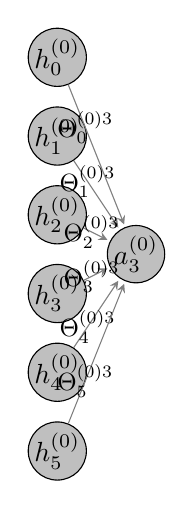
\begin{tikzpicture}[shorten >=1pt,-stealth,draw=black!50, node distance=\layersep]
    \tikzstyle{every pin edge}=[stealth-,shorten <=1pt]
    \tikzstyle{neuron}=[circle,draw=black,fill=black!25,minimum size=17pt,inner sep=0pt]
    \tikzstyle{input neuron}=[neuron, fill=gray!50];
    \tikzstyle{output neuron}=[neuron, fill=gray!50];
    \tikzstyle{hidden neuron}=[neuron, fill=gray!50];
    \tikzstyle{annot} = [text width=4em, text centered]

    % Draw the input layer nodes
    \foreach \name / \y in {1}
       	\pgfmathtruncatemacro{\m}{int(\y-1)}
    % This is the same as writing \foreach \name / \y in {1/1,2/2,3/3,4/4}
        \node[input neuron] (I-\name) at (0,-\y) {$h_{\m}^{(0)}$};


    \foreach \name / \y in {2,...,6}
       	\pgfmathtruncatemacro{\m}{int(\y-1)}
    % This is the same as writing \foreach \name / \y in {1/1,2/2,3/3,4/4}
        \node[input neuron] (I-\name) at (0,-\y) {$h_{\m}^{(0)}$};

    % Draw the hidden layer 1 nodes
    \foreach \name / \y in {4}
    	\pgfmathtruncatemacro{\m}{int(\y-1)}
        \path[yshift=0.5cm]
            node[hidden neuron] (H1-\name) at (\layersep,-\y cm) {$a_{\m}^{(0)}$};


 \path (I-1) edge node[pos=0.3,scale=0.9] {$\Theta^{(0)3}_0$} (H1-4);
 \path (I-2) edge node[pos=0.3,scale=0.9] {$\Theta^{(0)3}_1$} (H1-4);
 \path (I-3) edge node[pos=0.3,scale=0.9] {$\Theta^{(0)3}_2$} (H1-4);
 \path (I-4) edge node[pos=0.3,scale=0.9] {$\Theta^{(0)3}_3$} (H1-4);
 \path (I-5) edge node[pos=0.3,scale=0.9] {$\Theta^{(0)3}_4$} (H1-4);
 \path (I-6) edge node[pos=0.3,scale=0.9] {$\Theta^{(0)3}_5$} (H1-4);

\end{tikzpicture}
\caption{\label{fig:3}Weight averaging procedure.}
\end{center}
\end{figure}


Formally, the weight averaging procedure reads:

\begin{align}
a_{f}^{(t)(\nu)}&=\sum^{F_\nu-1+\epsilon}_{f'=0}\Theta^{(\nu)f}_{\,f'}h^{(t)(\nu)}_{f'}\;,
\end{align}
where $\nu\in\llbracket 0,N-1\rrbracket$, $t \in \llbracket0,T_{{\rm mb}}-1\rrbracket$ and $f\in \llbracket 0,F_{\nu+1}-1\rrbracket$. The $\epsilon$ is here to include or exclude a bias term. In practice, as we will be using batch-normalization, we can safely omit it ($\epsilon=0$ in all the following).

\section{Activation function}

The hidden neuron of each layer is defined as
\begin{align}
h_{f}^{(t)(\nu+1)}&=g\left(a_{f}^{(t)(\nu)}\right)\;,
\end{align}
where $\nu\in\llbracket 0,N-2\rrbracket$, $f\in \llbracket 0,F_{\nu+1}-1\rrbracket$ and as usual $t \in \llbracket0,T_{{\rm mb}}-1\rrbracket$. Here $g$ is an activation function -- the second main ingredient of a FNN -- whose non-linearity allow to predict arbitrary output data. In practice, $g$ is usually taken to be one of the functions described in the following subsections.


\subsection{The sigmoid function}

The sigmoid function takes its value in $]0,1[$ and reads
\begin{align}
g(x)&=\sigma(x)=\frac{1}{1+e^{-x}}\;.
\end{align}
Its derivative is
\begin{align}
\sigma'(x)&=\sigma(x)\left(1-\sigma(x)\right)\;.
\end{align}
This activation function is not much used nowadays (except in RNN-LSTM networks that we will present later in chapter \ref{sec:chapterRNN}).

\begin{figure}[H]
\begin{center}
\begin{tikzpicture}
\node at (0,0) {\includegraphics[scale=1]{sigmoid}};
\end{tikzpicture}
\end{center}
\caption{\label{fig:sigmoid} the sigmoid function and its derivative.}
\end{figure}

\subsection{The tanh function}

The tanh function takes its value in $]-1,1[$ and reads
\begin{align}
g(x)&=\tanh(x)=\frac{1-e^{-2x}}{1+e^{-2x}}\;.
\end{align}
Its derivative is
\begin{align}
\tanh'(x)&=1-\tanh^2(x)\;.
\end{align}
This activation function has seen its popularity drop due to the use of the activation function presented in the next section.

\begin{figure}[H]
\begin{center}
\begin{tikzpicture}
\node at (0,0) {\includegraphics[scale=1]{tanh2}};
\end{tikzpicture}
\end{center}
\caption{\label{fig:tanh} the tanh function and its derivative.}
\end{figure}

It is nevertherless still used in the standard formulation of the RNN-LSTM model (\ref{sec:chapterRNN}).

\subsection{The ReLU function}


The ReLU -- for Rectified Linear Unit -- function takes its value in $[0,+\infty[$ and reads
\begin{align}
g(x)&={\rm ReLU}(x)=\begin{cases}
      x & x\geq 0 \\
      0& x<0
   \end{cases}\;.
\end{align}
Its derivative is
\begin{align}
{\rm ReLU}'(x)&=\begin{cases}
      1 & x\geq 0 \\
      0 & x<0
   \end{cases}\;.
\end{align}

\begin{figure}[H]
\begin{center}
\begin{tikzpicture}
\node at (0,0) {\includegraphics[scale=1]{ReLU}};
\end{tikzpicture}
\end{center}
\caption{\label{fig:relu} the ReLU function and its derivative.}
\end{figure}


This activation function is the most extensively used nowadays. Two of its more common variants can also be found : the leaky ReLU and ELU -- Exponential Linear Unit. They have been introduced because the ReLU activation function tends to "kill" certain hidden neurons: once it has been turned off (zero value), it can never be turned on again.



\subsection{The leaky-ReLU function}


The leaky-ReLU --for Linear Rectified Linear Unit -- function takes its value in $]-\infty,+\infty[$ and is a slight modification of the ReLU that allows non-zero value for the hidden neuron whatever the $x$ value. It reads
\begin{align}
g(x)&={\rm lealy-ReLU}(x)=\begin{cases}
      x & x\geq 0 \\
      0.01\,x & x<0
   \end{cases}\;.
\end{align}
Its derivative is
\begin{align}
{\rm leaky-ReLU}'(x)&=\begin{cases}
      1 & x\geq 0 \\
      0.01 & x<0
   \end{cases}\;.
\end{align}

\begin{figure}[H]
\begin{center}
\begin{tikzpicture}
\node at (0,0) {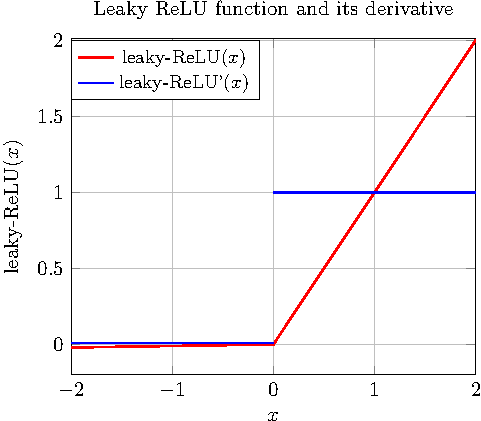
\includegraphics[scale=1]{lReLU}};
\end{tikzpicture}
\end{center}
\caption{\label{fig:lrelu} the leaky-ReLU function and its derivative.}
\end{figure}

A variant of the leaky-ReLU can also be found in the literature : the Parametric-ReLU, where the arbitrary $0.01$ in the definition of the leaky-ReLU is replaced by an $\alpha$ coefficient, that can be
computed via backpropagation.
\begin{align}
g(x)&={\rm Parametric-ReLU}(x)=\begin{cases}
      x & x\geq 0 \\
      \alpha\,x & x<0
   \end{cases}\;.
\end{align}
Its derivative is
\begin{align}
{\rm Parametric-ReLU}'(x)&=\begin{cases}
      1 & x\geq 0 \\
      \alpha & x<0
   \end{cases}\;.
\end{align}

\subsection{The ELU function}

The ELU --for Exponential Linear Unit -- function takes its value between $]-1,+\infty[$ and is inspired by the leaky-ReLU philosophy: non-zero values for all $x$'s. But it presents the advantage of being $\mathcal{C}^1$.
\begin{align}
g(x)&={\rm ELU}(x)=\begin{cases}
      x & x\geq 0 \\
      e^x-1 & x<0
   \end{cases}\;.
\end{align}
Its derivative is
\begin{align}
{\rm ELU}'(x)&=\begin{cases}
      1 & x\geq 0 \\
      e^x & x<0
   \end{cases}\;.
\end{align}


\begin{figure}[H]
\begin{center}
\begin{tikzpicture}
\node at (0,0) {\includegraphics[scale=1]{ELU}};
\end{tikzpicture}
\end{center}
\caption{\label{fig:elu} the ELU function and its derivative.}
\end{figure}

% From my experience, leay-relu is more than enough.


\section{FNN layers}

As illustrated in figure \ref{fig:1}, a regular FNN is composed by several specific layers. Let us explicit them one by one.



\subsection{Input layer}

The input layer is one of the two places where the data at disposal for the problem at hand come into place. In this chapter, we will be considering a input of size $F_0$, denoted $X^{(t)}_{f}$, with\footnote{
To train the FNN, we jointly compute the forward and backward pass for $T_{{\rm mb}}$ samples of the training set, with $T_{{\rm mb}}\ll T_{{\rm train}}$. In the following we will thus have $t\in \llbracket 0, T_{{\rm mb}}-1\rrbracket$.
}
 $t\in \llbracket 0, T_{{\rm mb}}-1\rrbracket$ (size of the mini-batch, more on that when we will be talking about gradient descent techniques), and $f \in \llbracket 0, F_0-1\rrbracket$. Given the problem at hand, a common procedure could be to center the input following the procedure
\begin{align}
\tilde{X}^{(t)}_{f}&=X^{(t)}_{f}-\mu_{f}\;,
\end{align}
with
\begin{align}
\mu_{f}&=\frac{1}{T_{{\rm train}}}\sum^{T_{{\rm train}}-1}_{t=0}X^{(t)}_{f}\;.
\end{align}
This correspond to compute the mean per data types over the training set. Following our notations, let us recall that
\begin{align}
X^{(t)}_{f}&=h^{(t)(0)}_{f}\;.
\end{align}

\subsection{Fully connected layer}

The fully connected operation is just the conjunction of the weight averaging and the activation procedure. Namely, $\forall \nu\in \llbracket 0,N-1 \rrbracket$
\begin{align}
a_{f}^{(t)(\nu)}&=\sum^{F_\nu-1}_{f'=0}\Theta^{(\nu)f}_{f'}h^{(t)(\nu)}_{f'}\;.\label{eq:Weightavg}
\end{align}
and $\forall \nu\in \llbracket 0,N-2 \rrbracket$
\begin{align}
h_{f}^{(t)(\nu+1)}&=g\left(a_{f}^{(t)(\nu)}\right)\;.
\end{align}
for the case where $\nu=N-1$, the activation function is replaced by an output function.



\subsection{Output layer}

The output of the FNN reads
 \begin{align}
h_{f}^{(t)(N)}&=o(a_{f}^{(t)(N-1)})\;,
\end{align}
where $o$ is called the output function. In the case of the Euclidean loss function, the output function is just the identity. In a classification task, $o$ is the softmax function.
\begin{align}
o\left(a^{(t)(N-1)}_f\right)&=\frac{e^{a^{(t)(N-1)}_f}}{\sum\limits^{F_{N-1}-1}_{f'=0}e^{a^{(t)(N-1)}_{f'}}}
\end{align}


\section{Loss function} \label{sec:FNNlossfunction}

The loss function evaluates the error performed by the FNN when it tries to estimate the data to be predicted (second place where the data make their appearance). For a regression problem, this is simply a mean square error (MSE) evaluation
\begin{align}
J(\Theta)&=\frac{1}{2T_{{\rm mb}}}\sum_{t=0}^{T_{{\rm mb}}-1}\sum_{f=0}^{F_N-1}
%
\left(y_f^{(t)}-h_{f}^{(t)(N)}\right)^2\;,
\end{align}
while for a classification task, the loss function is called the cross-entropy function
\begin{align}
J(\Theta)&=-\frac{1}{T_{{\rm mb}}}\sum_{t=0}^{T_{{\rm mb}}-1}\sum_{f=0}^{F_N-1}
%
\delta^f_{y^{(t)}}\ln h_{f}^{(t)(N)}\;,
\end{align}
and for a regression problem transformed into a classification one, calling $C$ the number of bins leads to
\begin{align}
J(\Theta)&=-\frac{1}{T_{{\rm mb}}}\sum_{t=0}^{T_{{\rm mb}}-1}\sum_{f=0}^{F_N-1}\sum_{c=0}^{C-1}
%
\delta^c_{y_f^{(t)}}\ln h_{fc}^{(t)(N)}\;.
\end{align}
For reasons that will appear clear when talking about the data sample used at each training step, we denote
\begin{align}
J(\Theta)&=\sum_{t=0}^{T_{{\rm mb}}-1}J_{{\rm mb}}(\Theta)\;.
\end{align}

\section{Regularization techniques}

On of the main difficulties when dealing with deep learning techniques is to get the deep neural network to train efficiently. To that end, several regularization techniques have been invented. We will review them in this section

\subsection{L2 regularization}

L2 regularization is the most common regularization technique that on can find in the literature. It amounts to add a regularizing term to the loss function in the following way
\begin{align}
J_{{\rm L2}}(\Theta)&=\lambda_{{\rm L2}} \sum_{\nu=0}^{N-1}\left\|\Theta^{(\nu)}\right\|^2_{{\rm L2}}
%
=\lambda_{{\rm L2}}\sum_{\nu=0}^{N-1}\sum_{f=0}^{F_{\nu+1}-1}\sum_{f'=0}^{F_\nu-1}
%
\left(\Theta^{(\nu)f'}_{f}\right)^2\;.\label{eq:l2reg}
\end{align}
This regularization technique is almost always used, but not on its own. A typical value of $\lambda_{{\rm L2}}$ is in the range $10^{-4}-10^{-2}$. Interestingly, this L2 regularization technique has a Bayesian interpretation: it is Bayesian inference with a Gaussian prior on the weights. Indeed, for a given $\nu$, the weight averaging procedure can be considered as
\begin{align}
a_{f}^{(t)(\nu)}&=\sum^{F_\nu-1}_{f'=0}\Theta^{(\nu)f}_{f'}h^{(t)(\nu)}_{f'}+\epsilon\;,
\end{align}
where $\epsilon$ is a noise term of mean $0$ and variance $\sigma^2$. Hence the following Gaussian likelihood for all values of $t$ and $f$:
\begin{align}
\mathcal{N}\left(a_{f}^{(t)(i)}\middle|\sum^{F_\nu-1}_{f'=0}\Theta^{(\nu)f}_{f'}h^{(t)(\nu)}_{f'},\sigma^2\right)\;.
\end{align}
Assuming all the weights to have a Gaussian prior of the form $\mathcal{N}\left(\Theta^{(\nu)f}_{f'}\middle|\lambda_{{\rm L2}}^{-1}\right)$ with the same parameter $\lambda_{{\rm L2}}$, we get the following expression
\begin{align}
\mathcal{P}&=
%
\prod_{t=0}^{T_{{\rm mb}}-1}\prod_{f=0}^{F_{\nu+1}-1}\left[\mathcal{N}\left(a_{f}^{(t)(\nu)}\middle|
%
\sum^{F_\nu-1}_{f'=0}\Theta^{(\nu)f}_{f'}h^{(t)(\nu)}_{f'},\sigma^2\right)
%
\prod_{f'=0}^{F_{\nu}-1}\mathcal{N}\left(\Theta^{(\nu)f}_{f'}
%
\middle|\lambda_{{\rm L2}}^{-1}\right)\right]\notag\\
%
&=\prod_{t=0}^{T_{{\rm mb}}-1}\prod_{f=0}^{F_{\nu+1}-1}\left[\frac{1}{\sqrt{2\pi \sigma^2}}
%
e^{-\frac{\left(a_{f}^{(t)(\nu)}-\sum^{F_i-1}_{f'=0}\Theta^{(\nu)f}_{f'}h^{(t)(\nu)}_{f'}\right)^2}{2\sigma^2}}
%
\prod_{f'=0}^{F_{\nu}-1}\sqrt{\frac{\lambda_{{\rm L2}}}{2\pi}}e^{-\frac{\left(\Theta^{(\nu)f}_{f'}\right)^2\lambda_{{\rm L2}}}{2}}\right] \;.
\end{align}
Taking the log of it and forgetting most of the constant terms leads to
\begin{align}
\mathcal{L}&\propto\frac{1}{T_{{\rm mb}}\sigma^2}
%
\sum_{t=0}^{T_{{\rm mb}}-1}\sum_{f=0}^{F_{\nu+1}-1}
%
\left(a_{f}^{(t)(\nu)}-\sum^{F_\nu-1}_{f'=0}\Theta^{(\nu)f}_{f'}h^{(t)(\nu)}_{f'}\right)^2
%
+\lambda_{{\rm L2}}\sum_{f=0}^{F_{\nu+1}-1}\sum_{f'=0}^{F_{\nu}-1}\left(\Theta^{(\nu)f}_{f'}\right)^2 \;,
\end{align}
and the last term is exactly the L2 regulator for a given $nu$ value (see formula (\ref{eq:l2reg})).

\subsection{L1 regularization}

L1 regularization amounts to replace the L2 norm by the L1 one in the L2 regularization technique
\begin{align}
J_{{\rm L1}}(\Theta)&=\lambda_{{\rm L1}} \sum_{\nu=0}^{N-1}\left\|\Theta^{(\nu)}\right\|_{{\rm L1}}
%
=\lambda_{{\rm L1}}\sum_{\nu=0}^{N-1}\sum_{f=0}^{F_{\nu+1}-1}\sum_{f'=0}^{F_\nu-1}
%
\left|\Theta^{(\nu)f}_{f'}\right|\;.
\end{align}
It can be used in conjunction with L2 regularization, but again these techniques are not sufficient on their own. A typical value of $\lambda_{{\rm L1}}$ is in the range $10^{-4}-10^{-2}$. Following the same line as in the previous section, one can show that L1 regularization is equivalent to Bayesian inference with a Laplacian prior on the weights
\begin{align}
\mathcal{F}\left(\Theta^{(\nu)f}_{f'}\middle| 0,\lambda_{{\rm L1}}^{-1}\right)&=
%
\frac{\lambda_{{\rm L1}}}{2}e^{-\lambda_{{\rm L1}}\left|\Theta^{(\nu)f}_{f'}\right|}\;.
\end{align}

\subsection{Clipping}

Clipping forbids the L2 norm of the weights to go beyond a pre-determined threshold $C$. Namely after having computed the update rules for the weights, if their L2 norm goes above $C$, it is pushed back to $C$
\begin{align}
{\rm if}\;\left\|\Theta^{(\nu)}\right\|_{{\rm L2}}>C \longrightarrow \Theta^{(\nu)f}_{f'}&=
%
\Theta^{(\nu)f}_{f'} \times \frac{C}{\left\|\Theta^{(\nu)}\right\|_{{\rm L2}}}\;.
\end{align}

This regularization technique avoids the so-called exploding gradient problem, and is mainly used in RNN-LSTM networks. A typical value of $C$ is in the range $10^{0}-10^{1}$. Let us now turn to the most efficient regularization techniques for a FNN: dropout and Batch-normalization.


\subsection{Dropout}

A simple procedure allows for better backpropagation performance for classification tasks: it amounts to stochastically drop some of the hidden units (and in some instances even some of the input variables) for each training example.

\begin{figure}[H]
\begin{center}
\begin{tikzpicture}[shorten >=1pt,-stealth,draw=black!50, node distance=\layersep]
    \tikzstyle{every pin edge}=[stealth-,shorten <=1pt]
    \tikzstyle{neuron}=[circle,draw=black,fill=black!25,minimum size=17pt,inner sep=0pt]
    \tikzstyle{input neuron}=[neuron, fill=gray!50];
    \tikzstyle{output neuron}=[neuron, fill=gray!50];
    \tikzstyle{dropout neuron}=[neuron, fill=black];
    \tikzstyle{hidden neuron}=[neuron, fill=gray!50];
    \tikzstyle{annot} = [text width=4em, text centered]

    % Draw the input layer nodes
    \foreach \name / \y in {1}
       	\pgfmathtruncatemacro{\m}{int(\y-1)}
    % This is the same as writing \foreach \name / \y in {1/1,2/2,3/3,4/4}
        \node[input neuron, pin=left:Bias] (I-\name) at (0,-\y) {$h_{\m}^{(0)}$};


    \foreach \name / \y in {2,3,4,6}
       	\pgfmathtruncatemacro{\m}{int(\y-1)}
    % This is the same as writing \foreach \name / \y in {1/1,2/2,3/3,4/4}
        \node[input neuron, pin=left:Input \#\y] (I-\name) at (0,-\y) {$h_{\m}^{(0)}$};

        \foreach \name / \y in {5}
       	\pgfmathtruncatemacro{\m}{int(\y-1)}
    % This is the same as writing \foreach \name / \y in {1/1,2/2,3/3,4/4}
        \node[dropout neuron] (I-\name) at (0,-\y) {$h_{\m}^{(0)}$};

    % Draw the hidden layer 1 nodes
    \foreach \name / \y in {1,2,3,5}
    	\pgfmathtruncatemacro{\m}{int(\y-1)}
        \path[yshift=0.5cm]
            node[hidden neuron] (H1-\name) at (\layersep,-\y cm) {$h_{\m}^{(1)}$};

    % Draw the hidden layer 1 nodes
    \foreach \name / \y in {4,6,7}
    	\pgfmathtruncatemacro{\m}{int(\y-1)}
        \path[yshift=0.5cm]
            node[dropout neuron] (H1-\name) at (\layersep,-\y cm) {$h_{\m}^{(1)}$};

    % Draw the hidden layer 1 node
    \foreach \name / \y in {1,3,5}
        \pgfmathtruncatemacro{\m}{int(\y-1)}
        \path[yshift=0.0cm]
            node[hidden neuron] (H2-\name) at (2*\layersep,-\y cm) {$h_{\m}^{(\nu)}$};

    % Draw the hidden layer 1 node
    \foreach \name / \y in {2,4,6}
        \pgfmathtruncatemacro{\m}{int(\y-1)}
        \path[yshift=0.0cm]
            node[dropout neuron] (H2-\name) at (2*\layersep,-\y cm) {$h_{\m}^{(\nu)}$};

    % Draw the output layer node
    \foreach \name / \y in {1,...,5}
        \path[yshift=-0.5cm]
    node[output neuron,pin={[pin edge={->}]right:Output \#\y}] (O-\name) at (3*\layersep,-\y cm) {$h_{\y}^{(N)}$};

    % Connect every node in the input layer with every node in the
    % hidden layer.
    \foreach \source in {1,2,3,4,6}
        \foreach \dest in {2,3,5}
            \path (I-\source) edge (H1-\dest);

     \foreach \source in {1,2,3,5}
       \foreach \dest in {3,5}
           \path (H1-\source) edge (H2-\dest);

    % Connect every node in the hidden layer with the output layer
    \foreach \source in {1,3,5}
       \foreach \dest in {1,...,5}
          \path (H2-\source) edge (O-\dest);

    % Annotate the layers
    \node[annot,above of=H1-1, node distance=1cm] (hl) {Hidden layer 1};
    \node[annot,left of=hl] {Input layer};
    \node[annot,right of=hl] (hm) {Hidden layer $\nu$};
    \node[annot,right of=hm] {Output layer};

    \node at ((1.5*\layersep,-3.5 cm) {$\bullet\bullet\bullet$};
    \node at ((2.5*\layersep,-3.5 cm) {$\bullet\bullet\bullet$};
\end{tikzpicture}
\caption{\label{fig:2}The neural network of figure \ref{fig:1} with dropout taken into account for both the hidden layers and the input. Usually, a different (lower) probability for turning off a neuron is adopted for the input than the one adopted for the hidden layers.}
\end{center}
\end{figure}


This amounts to do the following change: for $\nu\in \llbracket 1,N-1\rrbracket$
\begin{align}
h^{(\nu)}_{f}=\null&m_f^{(\nu)} g\left(a_f^{(\nu)}\right)
\end{align}
with $m_f^{(i)}$ following a $p$ Bernoulli distribution with usually $p=\frac15$ for the mask of the input layer and $p=\frac12$ otherwise. Dropout\cite{Srivastava:2014:DSW:2627435.2670313} has been the most successful regularization technique until the appearance of Batch Normalization.

\subsection{Batch Normalization}

Batch normalization\cite{Ioffe2015} amounts to jointly normalize the mini-batch set per data types, and does so at each input of a FNN layer. In the original paper, the authors argued that this step should be done after the convolutional layers, but in practice it has been shown to be more efficient after the non-linear step. In our case, we will thus consider $\forall i \in \llbracket 0,N-2\rrbracket$
\begin{align}
\tilde{h}_{f}^{(t)(\nu)}&=\frac{h_{f}^{(t)(\nu+1)}-\hat{h}_{f}^{(\nu)}}
%
{\sqrt{\left(\hat{\sigma}_{f}^{(\nu)}\right)^2+\epsilon}}\;,
\end{align}
with
\begin{align}
\hat{h}_{f}^{(\nu)}&=
%
\frac{1}{T_{{\rm mb}}}\sum^{T_{{\rm mb}}-1}_{t=0}h_{f}^{(t)(\nu+1)}\\
%
\left(\hat{\sigma}_{f}^{(\nu)}\right)^2&=\frac{1}{T_{{\rm mb}}}\sum^{T_{{\rm mb}}-1}_{t=0}
%
\left(h_{f}^{(t)(\nu+1)}-\hat{h}_{f}^{(\nu)}\right)^2\;.
\end{align} To make sure that this transformation can represent the identity transform, we add two additional parameters $(\gamma_f,\beta_f)$ to the model
\begin{align}
y^{(t)(\nu)}_{f}&=\gamma^{(\nu)}_f\,\tilde{h}_{f}^{(t)(\nu)}+\beta^{(\nu)}_f
%
=\tilde{\gamma}^{(\nu)}_f\,h_{f}^{(t)(\nu)}+\tilde{\beta}^{(\nu)}_f\;.
\end{align}
The presence of the $\beta^{(\nu)}_f$ coefficient is what pushed us to get rid of the bias term, as it is naturally included in batchnorm. During training, one must compute a running sum for the mean and the variance, that will serve for the evaluation of the cross-validation and the test set (calling $e$ the number of iterations/epochs)
\begin{align}
\mathbb{E}\left[h_{f}^{(t)(\nu+1)}\right]_{e+1} &=
%
\frac{e\mathbb{E}\left[h_{f}^{(t)(\nu)}\right]_{e}+\hat{h}_{f}^{(\nu)}}{e+1}\;,\\
%
\mathbb{V}ar\left[h_{f}^{(t)(\nu+1)}\right]_{e+1} &=
%
\frac{e\mathbb{V}ar\left[h_{f}^{(t)(\nu)}\right]_{e}+\left(\hat{\sigma}_{f}^{(\nu)}\right)^2}{e+1}
\end{align}
and what will be used at test time is
\begin{align}
\mathbb{E}\left[h_{f}^{(t)(\nu)}\right]&=\mathbb{E}\left[h_{f}^{(t)(\nu)}\right]\;,&
%
\mathbb{V}ar\left[h_{f}^{(t)(\nu)}\right]&=
%
\frac{T_{{\rm mb}}}{T_{{\rm mb}}-1}\mathbb{V}ar\left[h_{f}^{(t)(\nu)}\right]\;.
\end{align}
so that at test time
\begin{align}
y^{(t)(\nu)}_{f}&=\gamma^{(\nu)}_f\,\frac{h_{f}^{(t)(\nu)}-E[h_{f}^{(t)(\nu)}]}{\sqrt{Var\left[h_{f}^{(t)(\nu)}\right]+\epsilon}}+\beta^{(\nu)}_f\;.
\end{align}

In practice, and as advocated in the original paper, on can get rid of dropout without loss of precision when using batch normalization. We will adopt this convention in the following.


\section{Backpropagation}

Backpropagation\cite{LeCun:1998:EB:645754.668382} is the standard technique to decrease the loss function error so as to correctly predict what one needs. As it name suggests, it amounts to backpropagate through the FNN the error performed at the output layer, so as to update the weights. In practice, on has to compute a bunch of gradient terms, and this can be a tedious computational task. Nevertheless, if performed correctly, this is the most useful and important task that one can do in a FN. We will therefore detail how to compute each weight (and Batchnorm coefficients) gradients in the following.

\subsection{Backpropagate through Batch Normalization} \label{sec:Backpropbatchnorm}

Backpropagation introduces a new gradient
\begin{align}
\delta^f_{f'}J^{(tt')(\nu)}_{f}&=\frac{\partial y^{(t')(\nu)}_{f'}}{\partial h_{f}^{(t)(\nu+1)}}\;.
\end{align}
we show in appendix \ref{sec:appenbatchnorm} that
\begin{align}
J^{(tt')(\nu)}_{f}&=\tilde{\gamma}^{(\nu)}_f\ \left[\delta^{t'}_t-
%
\frac{1+\tilde{h}_{f}^{(t')(\nu)}\tilde{h}_{f}^{(t)(\nu)}}{T_{{\rm mb}}}\right]\;.
\end{align}


\subsection{error updates}


To backpropagate the loss error through the FNN, it is very useful to compute a so-called error rate
\begin{align}
\delta^{(t)(\nu)}_f&= \frac{\partial }{\partial a_{f}^{(t)(\nu)}}J(\Theta)\;,
\end{align}
We show in Appendix \ref{sec:appenbplayers} that $\forall \nu \in \llbracket 0,N-2\rrbracket$
\begin{align}
\delta^{(t)(\nu)}_f&=g'\left(a_{f}^{(t)(\nu)}\right)
%
\sum_{t'=0}^{T_{{\rm mb}}-1}\sum_{f'=0}^{F_{\nu+1}-1}\Theta^{(\nu+1)f'}_{f}J^{(tt')(\nu)}_{f} \delta^{(t')(\nu+1)}_{f'}\;,
\end{align}
the value of $\delta^{(t)(N-1)}_f$ depends on the loss used. We show also in appendix \ref{sec:appenbpoutput} that for the MSE loss function
\begin{align}
\delta^{(t)(N-1)}_f&= \frac{1}{T_{{\rm mb}}}\left(h_{f}^{(t)(N)}-y_f^{(t)}\right)\;,
\end{align}
and for the cross entropy loss function
\begin{align}
\delta^{(t)(N-1)}_{f}&= \frac{1}{T_{{\rm mb}}}\left(h_{f}^{(t)(N)}-\delta^f_{y^{(t)}}\right)\;.
\end{align}
To unite the notation of chapters \ref{sec:chapterFNN}, \ref{sec:chapterCNN} and \ref{sec:chapterRNN}, we will call
\begin{align}
\mathcal{H}^{(t)(\nu+1)}_{ff'}&=g'\left(a_{f}^{(t)(\nu)}\right)\Theta^{(\nu+1)f'}_{f}\;,
\end{align}
so that the update rule for the error rate reads
\begin{align}
\delta^{(t)(\nu)}_f&=
%
\sum_{t'=0}^{T_{{\rm mb}}-1}J^{(tt')(\nu)}_{f}\sum_{f'=0}^{F_{\nu+1}-1}\mathcal{H}^{(t)(\nu+1)}_{ff'} \delta^{(t)(\nu+1)}_{f'}\;.
\end{align}

\subsection{Weight update}

Thanks to the computation of the error rates, the derivation of the error rate is straightforward. We indeed get $\forall \nu \in \llbracket 1,N-1\rrbracket$
\begin{align}
\Delta^{\Theta(\nu)f}_{f'}&=\frac{1}{T_{{\rm mb}}}\sum_{t=0}^{T_{{\rm mb}}-1}
%
\sum^{F_{\nu+1}-1}_{f^{''}=0}\sum^{F_\nu}_{f^{'''}=0}\frac{\partial\Theta^{(\nu)f^{''}}_{f^{'''}}
%
}{\partial \Theta^{(\nu)f}_{f'}}y^{(t)(\nu-1)}_{f^{'''}}\delta^{(t)(\nu)}_{f^{''}}
%
=\sum_{t=0}^{T_{{\rm mb}}-1}\delta^{(t)(\nu)}_f y^{(t)(\nu-1)}_{f'}\;.
\end{align}
and
\begin{align}
\Delta^{\Theta(0)f}_{f'}&=\sum_{t=0}^{T_{{\rm mb}}-1}\delta^{(t)(0)}_f h^{(t)(0)}_{f'}\;.
\end{align}

\subsection{Coefficient update}

The update rule for the Batchnorm coefficient can easily be computed thanks to the error rate. It reads
\begin{align}
\Delta_f^{\gamma(\nu)}&=\sum_{t=0}^{T_{{\rm mb}}-1}\sum_{f'=0}^{F_{\nu+1}-1}
%
\frac{\partial a^{(t)(\nu+1)}_{f'}}{\partial\gamma_f^{(i)}}\delta^{(t)(\nu+1)}_{f'}
%
=\sum_{t=0}^{T_{{\rm mb}}-1}\sum_{f'=0}^{F_{\nu+1}-1}
%
\Theta^{(\nu+1)f'}_{f}\tilde{h}^{(t)(i)}_{f}\delta^{(t)(\nu+1)}_{f'}\;,\\
%
\Delta_f^{\beta(\nu)}&=\sum_{t=0}^{T_{{\rm mb}}-1}\sum_{f'=0}^{F_{\nu+1}-1}
%
\frac{\partial a^{(t)(\nu+1)}_{f'}}{\partial\beta_f^{(i)}}\delta^{(t)(\nu+1)}_{f'}
%
=\sum_{t=0}^{T_{{\rm mb}}-1}\sum_{f'=0}^{F_{\nu+1}-1}\Theta^{(\nu+1)f'}_{f}\delta^{(t)(\nu+1)}_{f'}\;,
\end{align}


\section{Which data sample to use for gradient descent?}

From the beginning we have denoted $T_{{\rm mb}}$ the sample of the data from which we train our model. This procedure is repeated a large number of time (each time is called an epoch). But in the literature there exists three way to sample from the data: Full-batch, Stochastic and Mini-batch gradient descent. We explicit these terms in the following sections.

\subsection{Full-batch}

Full-batch takes the whole training set at each epoch, such that the loss function reads
\begin{align}
J(\Theta)&=\sum_{t=0}^{T_{{\rm train}}-1}J_{{\rm train}}(\Theta)\;.
\end{align}
This choice has the advantage to be numerically stable, but it so costly in computation time that it is rarely if ever used.

\subsection{Stochastic Gradient Descent (SGD)}

SGD amounts to take only one exemplary of the training set at each epoch
\begin{align}
J(\Theta)&=J_{{\rm SGD}}(\Theta)\;.
\end{align}
This choice leads to faster computations, but is so numerically unstable that the most standard choice by far is Mini-batch gradient descent.

\subsection{Mini-batch}

Mini-batch gradient descent is a compromise between stability and time efficiency, and is the middle-ground between Full-batch and Stochastic gradient descent: $1\ll T_{{\rm mb}}\ll T_{{\rm train}}$. Hence
\begin{align}
J(\Theta)&=\sum_{t=0}^{T_{{\rm mb}}-1}J_{{\rm mb}}(\Theta)\;.
\end{align}
All the calculations in this note have been performed using this gradient descent technique.

\section{Gradient optimization techniques}

Once the gradients for backpropagation have been computed, the question of how to add them to the existing weights arise. The most natural choice would be to take
\begin{align}
\Theta^{(\nu)f}_{f'}&=\Theta^{(\nu)f}_{f'}-\eta\Delta^{\Theta(i)f}_{f'}\;.
\end{align}
where $\eta$ is a free parameter that is generally initialized thanks to cross-validation. It can also be made epoch dependent (with usually a slow exponentially decaying behaviour). When using Mini-batch gradient descent, this update choice for the weights presents the risk of having the loss function being stuck in a local minimum. Several method have been invented to prevent this risk. We are going to review them in the next sections.


\subsection{Momentum}

Momentum\cite{QIAN1999145} introduces a new vector $v_{{\rm e}}$ and can be seen as keeping a memory of what where the previous updates at prior epochs. Calling $e$ the number of epochs and forgetting the $f,f',\nu$ indices for the gradients to ease the notations, we have
\begin{align}
v_{{\rm e}}&=\gamma v_{{\rm e-1}}+\eta \Delta^{\Theta}\;,
\end{align}
and the weights at epoch $e$ are then updated as
\begin{align}
\Theta_e&=\Theta_{e-1}-v_{{\rm e}}\;.
\end{align}
$\gamma$ is a new parameter of the model, that is usually set to $0.9$ but that could also be fixed thanks to cross-validation.

\subsection{Nesterov accelerated gradient}

Nesterov accelerated gradient\cite{nesterov1983method} is a slight modification of the momentum technique that allows the gradients to escape from local minima. It amounts to take
\begin{align}
v_{{\rm e}}&=\gamma v_{{\rm e-1}}+\eta \Delta^{\Theta-\gamma v_{{\rm e-1}}}\;,
\end{align}
and then again
\begin{align}
\Theta_e&=\Theta_{e-1}-v_{{\rm e}}\;.
\end{align}
Until now, the parameter $\eta$ that controls the magnitude of the update has been set globally. It would be nice to have a fine control of it, so that different weights can be updated with different magnitudes.

\subsection{Adagrad}

Adagrad\cite{Duchi:2011:ASM:1953048.2021068} allows to fine tune the different gradients by having individual learning rates $\eta$. Calling for each value of $f,f',i$
\begin{align}
v_{{\rm e}}&=\sum_{e'=0}^{e-1} \left(\Delta^{\Theta}_{e'}\right)^2\;,
\end{align}
the update rule then reads
\begin{align}
\Theta_e&=\Theta_{e-1}-\frac{\eta}{\sqrt{v_{{\rm e}}+\epsilon}}\Delta^{\Theta}_{e}\;.
\end{align}
One advantage of Adagrad is that the learning rate $\eta$ can be set once and for all (usually to $10^{-2}$) and does not need to be fine tune via cross validation anymore, as it is individually adapted to each weight via the $v_{{\rm e}}$ term. $\epsilon$ is here to avoid division by 0 issues, and is usually set to $10^{-8}$.

\subsection{RMSprop}

Since in Adagrad one adds the gradient from the first epoch, the weight are forced to monotonically decrease. This behaviour can be smoothed via the Adadelta technique, which takes
\begin{align}
v_{{\rm e}}&=\gamma v_{{\rm e-1}}+(1-\gamma )\Delta^{\Theta}_{e}\;,
\end{align}
with $\gamma$ a new parameter of the model, that is usually set to $0.9$. The Adadelta update rule then reads as the Adagrad one
\begin{align}
\Theta_e&=\Theta_{e-1}-\frac{\eta}{\sqrt{v_{{\rm e}}+\epsilon}}\Delta^{\Theta}_{e}\;.
\end{align}
$\eta$ can be set once and for all (usually to $10^{-3}$).

\subsection{Adadelta}

Adadelta\cite{journals/corr/abs-1212-5701} is an extension of RMSprop, that aims at getting rid of the $\eta$ parameter. To do so, a new vector update is introduced
\begin{align}
m_{{\rm e}}&=\gamma m_{{\rm e-1}}+(1-\gamma )
%
\left(\frac{\sqrt{m_{{\rm e-1}}+\epsilon}}{\sqrt{v_{{\rm e}}+\epsilon}}\Delta^{\Theta}_{e}\right)^2\;,
\end{align}
and the new update rule for the weights reads
\begin{align}
\Theta_e&=\Theta_{e-1}-\frac{\sqrt{m_{{\rm e-1}}+\epsilon}}{\sqrt{v_{{\rm e}}+\epsilon}}\Delta^{\Theta}_{e}\;.
\end{align}
The learning rate has been completely eliminated from the update rule, but the procedure for doing so is ad hoc. The next and last optimization technique presented seems more natural and is the default choice on a number of deep learning algorithms.
\subsection{Adam}

Adam\cite{Kingma2014} keeps track of both the gradient and its square via two epoch dependent vectors
\begin{align}
m_{{\rm e}}&= \beta_1 m_{{\rm e-1}}+ (1-\beta_1)\Delta^{\Theta}_{e}\;,&
%
v_{{\rm e}}&= \beta_2 v_{{\rm e}}+ (1-\beta_2)\left(\Delta^{\Theta}_{e}\right)^2\;,
\end{align}
with $\beta_1$ and $\beta_2$ parameters usually respectively set to $0.9$ and $0.999$. But the robustness and great strength of Adam is that it makes the whole learning process weakly dependent of their precise value. To avoid numerical problems during the first steps, these vector are rescaled
\begin{align}
\hat{m}_{{\rm e}}&= \frac{m_{{\rm e}}}{1-\beta_1^{e}}\;,&
%
\hat{v}_{{\rm e}}&= \frac{v_{{\rm e}}}{1-\beta_2^{e}}\;.
\end{align}
before entering into the update rule
\begin{align}
\Theta_e&=\Theta_{e-1}-\frac{\eta }{\sqrt{\hat{v}_{{\rm e}}+\epsilon}}\hat{m}_{{\rm e}}\;.
\end{align}
This is the optimization technique implicitly used throughout this note, alongside with a learning rate decay
\begin{align}
\eta_e&=e^{-\alpha_0}\eta_{e-1}\;,
\end{align}
$\alpha_0$ determined by cross-validation, and $\eta_0$ usually initialized in the range $10^{-3}-10^{-2}$.

\section{Weight initialization}

Without any regularization, training a neural network can be a daunting task because of the fine-tuning of the weight initial conditions. This is one of the reasons why neural networks have experienced out of mode periods. Since dropout and Batch normalization, this issue is less pronounced, but one should not initialize the weight in a symmetric fashion (all zero for instance), nor should one initialize them too large. A good heuristic is
\begin{align}
\left[\Theta^{(\nu)f'}_f\right]_{{\rm init}}&=\sqrt{\frac{6}{F_\nu+F_{\nu+1}}}\times\mathcal{N}(0,1)\;.
\end{align}

\begin{subappendices}
\section{Backprop through the output layer} \label{sec:appenbpoutput}

Recalling the MSE loss function
\begin{align}
J(\Theta)&=\frac{1}{2T_{{\rm mb}}}\sum_{t=0}^{T_{{\rm mb}}-1}\sum_{f=0}^{F_N-1}
%
\left(y_f^{(t)}-h_{f}^{(t)(N)}\right)^2\;,
\end{align}
we instantaneously get
\begin{align}
\delta^{(t)(N-1)}_f&= \frac{1}{T_{{\rm mb}}}\left(h_{f}^{(t)(N)}-y_f^{(t)}\right)\;.
\end{align}
Things are more complicated for the cross-entropy loss function of a regression problem transformed into a multi-classification task.
Assuming that we have $C$ classes for all the values that we are trying to predict, we get
\begin{align}
\delta^{(t)(N-1)}_{fc}&= \frac{\partial }{\partial a_{fc}^{(t)(N-1)}}J(\Theta)
%
=\sum_{t'=0}^{T_{{\rm mb}}-1}\sum_{f'=0}^{F_N-1}\sum_{d=0}^{C-1}
%
\frac{\partial h_{f'd}^{(t')(N)}}{\partial a_{fc}^{(t)(N-1)}}
%
 \frac{\partial }{\partial h_{f'd}^{(t')(N)}}J(\Theta)\;.
\end{align}
Now
\begin{align}
 \frac{\partial }{\partial h_{f'd}^{(t')(N)}}J(\Theta)&=-\frac{\delta^{d}_{ y_{f'}^{(t')}}}{T_{{\rm mb}} h_{f'd}^{(t')(N)}}\;,
\end{align}
and
\begin{align}
\frac{\partial h_{f'd}^{(t')(N)}}{\partial a_{fc}^{(t)(N-1)}}&=
%
\delta^f_{f'}\delta^{t}_{t'} \left(\delta^c_d h_{fc}^{(t)(N)}- h_{fc}^{(t)(N)} h_{fd}^{(t)(N)}\right)\;,
\end{align}
so that
\begin{align}
\delta^{(t)(N-1)}_{fc}&=-\frac{1}{T_{{\rm mb}}} \sum_{d=0}^{C-1}\frac{\delta^{d}_{ y_f^{(t)}}}{h_{fd}^{(t)(N)}}
%
\left(\delta^c_d h_{fc}^{(t)(N)}- h_{fc}^{(t)(N)} h_{fd}^{(t)(N)}\right)\notag\\
%
&=\frac{1}{T_{{\rm mb}}}\left( h_{fc}^{(t)(N)}-\delta^{c}_{ y_f^{(t)}}\right)\;.
\end{align}
For a true classification problem, we easily deduce
\begin{align}
\delta^{(t)(N-1)}_{fc}&=\frac{1}{T_{{\rm mb}}}\left( h_{f}^{(t)(N)}-\delta^{f}_{ y^{(t)}}\right)\;.
\end{align}

\section{Backprop through hidden layers} \label{sec:appenbplayers}

To go further we need
\begin{align}
\delta^{(t)(\nu)}_f&= \frac{\partial }{\partial a_{f}^{(t)(\nu)}}J^{(t)}(\Theta)=
%
\sum_{t'=0}^{T_{{\rm mb}}-1}\sum_{f'=0}^{F_{\nu+1}-1}
%
 \frac{\partial a_{f'}^{(t')(\nu+1)}}{\partial a_{f}^{(t)(\nu)}} \delta^{(t')(\nu+1)}_{f'}\notag\\
%
&=\sum_{t'=0}^{T_{{\rm mb}}-1}\sum_{f'=0}^{F_{\nu+1}-1}\sum^{F_\nu}_{f''=0}\Theta^{(\nu+1)f'}_{f''}
%
\frac{\partial y^{(t')(\nu)}_{f''} }{\partial a_{f}^{(t)(\nu)}} \delta^{(t')(\nu+1)}_{f'}\notag\\
%
&=\sum_{t'=0}^{T_{{\rm mb}}-1}\sum_{f'=0}^{F_{\nu+1}-1}\sum^{F_\nu}_{f''=0}\Theta^{(\nu+1)f'}_{f''}
%
\frac{\partial y^{(t')(\nu)}_{f''} }{\partial h_{f}^{(t)(\nu+1)}}
%
g'\left(a_{f}^{(t)(\nu)}\right) \delta^{(t')(\nu+1)}_{f'}\;,
\end{align}
so that
\begin{align}
\delta^{(t)(\nu)}_f&=g'\left(a_{f}^{(t)(\nu)}\right)
%
\sum_{t'=0}^{T_{{\rm mb}}-1}\sum_{f'=0}^{F_{\nu+1}-1}\Theta^{(\nu+1)f'}_{f}J^{(tt')(\nu)}_{f} \delta^{(t)(\nu+1)}_{f'}\;,
\end{align}


\section{Backprop through BatchNorm} \label{sec:appenbatchnorm}


We saw in section \ref{sec:Backpropbatchnorm} that batch normalization implies among other things to compute the following gradient.
\begin{align}
\frac{\partial y^{(t')(\nu)}_{f'}}{\partial h_{f}^{(t)(\nu+1)}}&=
%
\gamma^{(\nu)}_f\frac{\partial \tilde{h}_{f'}^{(t)(\nu)}}{\partial h_{f}^{(t)(\nu+1)}}\;.
\end{align}
We propose to do just that in this section. Firstly
\begin{align}
\frac{\partial h^{(t')(\nu+1)}_{f'}}{\partial h_{f}^{(t)(\nu+1)}}&=\delta^{t'}_t\delta^{f'}_f\;,&
%
\frac{\partial \hat{h}_{f'}^{(\nu)}}{\partial h_{f}^{(t)(\nu+1)}}&=\frac{\delta^{f'}_f}{T_{{\rm mb}}}\;.
\end{align}
Secondly
\begin{align}
\frac{\partial \left(\hat{\sigma}_{f'}^{(\nu)}\right)^2}{\partial h_{f}^{(t)(\nu+1)}}&=
%
\frac{2\delta^{f'}_f}{T_{{\rm mb}}}\left(h_{f}^{(t)(\nu+1)}-\hat{h}_{f}^{(\nu)}\right)\;,
\end{align}
so that we get
\begin{align}
\frac{\partial \tilde{h}_{f'}^{(t)(\nu)}}{\partial h_{f}^{(t)(\nu+1)}}&=
%
\frac{\delta^{f'}_f}{T_{{\rm mb}}}\left[\frac{T_{{\rm mb}}\delta^{t'}_t-1}
%
{\left(\left(\hat{\sigma}_{f}^{(\nu)}\right)^2+\epsilon\right)^\frac12}-
%
\frac{\left(h_{f}^{(t')(\nu+1)}-\hat{h}_{f}^{(\nu)}\right)\left(h_{f}^{(t)(\nu+1)}-\hat{h}_{f}^{(\nu)}\right)}
%
{\left(\left(\hat{\sigma}_{f}^{(\nu)}\right)^2+\epsilon\right)^\frac32}\right]\notag\\
%
&=\frac{\delta^{f'}_f}{\left(\left(\hat{\sigma}_{f}^{(\nu)}\right)^2+\epsilon\right)^\frac12}
%
\left[\delta^{t'}_t-
%
\frac{1+\tilde{h}_{f}^{(t')(\nu)}\tilde{h}_{f}^{(t)(\nu)}}{T_{{\rm mb}}}\right]\;.
\end{align}
To ease the notation recall that we denoted
\begin{align}
\tilde{\gamma}^{(\nu)}_f&=
%
\frac{\gamma^{(\nu)}_f}{\left(\left(\hat{\sigma}_{f}^{(\nu)}\right)^2+\epsilon\right)^\frac12}\;.
\end{align}
%
%
so that
\begin{align}
\frac{\partial y_{f'}^{(t)(\nu)}}{\partial h_{f}^{(t)(\nu+1)}}&=
%
\tilde{\gamma}^{(\nu)}_f \delta^{f'}_f\left[\delta^{t'}_t-
%
\frac{1+\tilde{h}_{f}^{(t')(\nu)}\tilde{h}_{f}^{(t)(\nu)}}{T_{{\rm mb}}}\right]\;.
\end{align}



\section{FNN ResNet (non standard presentation)} \label{sec:ResnetFNN}

The state of the art architecture of convolutional neural networks (CNN, to be explained in chapter \ref{sec:chapterCNN}) is called ResNet\cite{He2015}. Its name comes from its philosophy: each hidden layer output $y$ of the network is a small -- hence the term residual -- modification of its input ($y=x+F(x)$), instead of a total modification ($y=H(x)$) of its input $x$. This philosophy can be imported to the FNN case. Representing the operations of weight averaging, activation function and batch normalization in the following way

\begin{figure}[H]
\begin{center}
\begin{tikzpicture}
\node at (0,0) {\includegraphics[scale=1]{fc_equiv}};
\end{tikzpicture}
\end{center}
\caption{\label{fig:fc_equiv} Schematic representation of one FNN fully connected layer.}
\end{figure}

In its non standard form presented in this section, the residual operation amounts to add a skip connection to two consecutive full layers


\begin{figure}[H]
\begin{center}
\begin{tikzpicture}
\node at (0,0) {\includegraphics[scale=1]{fc_resnet_2}};
\end{tikzpicture}
\end{center}
\caption{\label{fig:fc_resnet_2} Residual connection in a FNN.}
\end{figure}

Mathematically, we had before (calling the input $y^{(t)(\nu-1)}$)

\begin{align}
y_{f}^{(t)(\nu+1)}&=\gamma_f^{(\nu+1)}\tilde{h}_f^{(t)(\nu+2)}+\beta_f^{(\nu+1)}\;,&
%
a_{f}^{(t)(\nu+1)}&=\sum^{F_{\nu}-1}_{f'=0}\Theta^{(\nu+1)f}_{f'}y_{f}^{(t)(\nu)}\notag\\
%
y_{f}^{(t)(\nu)}&=\gamma_f^{(\nu)}\tilde{h}_f^{(t)(\nu+1)}+\beta_f^{(\nu)}\;,&
%
a_{f}^{(t)(\nu)}&=\sum^{F_{\nu-1}-1}_{f'=0}\Theta^{(\nu)f}_{f'}y_{f}^{(t)(\nu-1)}\;,
\end{align}
as well as $h^{(t)(\nu+2)}_f=g\left(a_{f}^{(t)(\nu+1)}\right)$ and $h^{(t)(\nu+1)}_f=g\left(a_{f}^{(t)(\nu)}\right)$. In ResNet, we now have the slight modification
\begin{align}
y_{f}^{(t)(\nu+1)}&=\gamma_f^{(\nu+1)}\tilde{h}_f^{\nu+2}+\beta_f^{(\nu+1)}+y^{(t)(\nu-1)}_{f}\;.
\end{align}
The choice of skipping two and not just one layer has become a standard for empirical reasons, so as the decision not to weight the two paths (the trivial skip one and the two FNN layer one) by a parameter to be learned by backpropagation
\begin{align}
y_{f}^{(t)(\nu+1)}&=\alpha\left(\gamma_f^{(\nu+1)}\tilde{h}_f^{(t)(\nu+2)}+\beta_f^{(\nu+1)}\right)
%
+\left( 1-\alpha\right)y^{(t)(\nu-1)}_{f'}\;.
\end{align}
This choice is called highway nets\cite{citeulike:14070430}, and it remains to be theoretically understood why it leads to worse performance than ResNet, as the latter is a particular instance of the former. Going back to the ResNet backpropagation algorithm, this changes the gradient through the skip connection in the following way
\begin{align}
\delta^{(t)(\nu-1)}_f&=
%
\sum_{t'=0}^{T_{{\rm mb}}-1}\sum_{f'=0}^{F_{\nu}-1}
%
 \frac{\partial a_{f'}^{(t')(\nu)}}{\partial a_{f}^{(t)(\nu-1)}} \delta^{(t')(\nu)}_{f'}
 %
+\sum_{t'=0}^{T_{{\rm mb}}-1}\sum_{f'=0}^{F_{\nu+2}-1}
%
 \frac{\partial a_{f'}^{(t')(\nu+2)}}{\partial a_{f}^{(t)(\nu-1)}} \delta^{(t')(\nu+2)}_{f'}\notag\\
%
&=\sum_{t'=0}^{T_{{\rm mb}}-1}\sum_{f'=0}^{F_{\nu}-1}\sum^{F_{\nu-1}-1}_{f''=0}\Theta^{(\nu)f'}_{f''}
%
\frac{\partial y^{(t')(\nu-1)}_{f''} }{\partial a_{f}^{(t)(\nu-1)}} \delta^{(t')(\nu)}_{f'}\notag\\
%
&+\sum_{t'=0}^{T_{{\rm mb}}-1}\sum_{f'=0}^{F_{\nu+2}-1}\sum^{F_{\nu-1}-1}_{f''=0}\Theta^{(\nu+2)f'}_{f''}
%
\frac{\partial y^{(t')(\nu+1)}_{f''} }{\partial a_{f}^{(t)(\nu-1)}} \delta^{(t')(\nu+2)}_{f'}\notag\\
%
&=g'\left(a_{f}^{(t)(\nu-1)}\right)
%
\sum_{t'=0}^{T_{{\rm mb}}-1}\sum_{f'=0}^{F_{\nu}-1}\sum^{F_{\nu-1}-1}_{f''=0}\Theta^{(\nu)f'}_{f''}
%
J^{(tt')(\nu)}_{f} \delta^{(t')(\nu)}_{f'}\notag\\
%
&+g'\left(a_{f}^{(t)(\nu-1)}\right)
%
\sum_{t'=0}^{T_{{\rm mb}}-1}\sum_{f'=0}^{F_{\nu+2}-1}\sum^{F_{\nu-1}-1}_{f''=0}\Theta^{(\nu+2)f'}_{f''}
%
J^{(tt')(\nu)}_{f} \delta^{(t')(\nu+2)}_{f'}\;,
\end{align}
so that
\begin{align}
\delta^{(t)(\nu-1)}_f&=g'\left(a_{f}^{(t)(\nu-1)}\right)
%
\sum_{t'=0}^{T_{{\rm mb}}-1}\sum^{F_{\nu-1}-1}_{f''=0}J^{(tt')(\nu)}_{f}\notag\\
%
&\times\left[\sum_{f'=0}^{F_{\nu}-1}\Theta^{(\nu)f'}_{f''}\delta^{(t')(\nu)}_{f'}+
%
\sum_{f'=0}^{F_{\nu+2}-1}\Theta^{(\nu+2)f'}_{f''}\delta^{(t')(\nu+2)}_{f'}\right]\;.
\end{align}

This formulation has one advantage: it totally preserves the usual FNN layer structure of a weight averaging (WA) followed by an activation function (AF) and then a batch normalization operation (BN). It nevertheless has one disadvantage: the backpropagation gradient does not really flow smoothly from one error rate to the other. In the following section we will present the standard ResNet formulation of that takes the problem the other way around : it allows the gradient to flow smoothly at the cost of "breaking" the natural FNN building block.

\section{FNN ResNet (more standard presentation)} \label{sec:ResnetFNN2}

\begin{figure}[H]
\begin{center}
\begin{tikzpicture}
\node at (0,0) {\includegraphics[scale=1]{fc_resnet_3}};
\end{tikzpicture}
\end{center}
\caption{\label{fig:fc_resnet_3} Residual connection in a FNN, trivial gradient flow through error rates.}
\end{figure}

In the more standard form of ResNet, the skip connections reads
\begin{align}
 a_{f}^{(t)(\nu+2)}&= a_{f}^{(t)(\nu+2)}+ a_{f}^{(t)(\nu)}\;,
\end{align}
and the updated error rate reads
\begin{align}
\delta^{(t)(\nu)}_f&=g'\left(a_{f}^{(t)(\nu)}\right)
%
\sum_{t'=0}^{T_{{\rm mb}}-1}\sum^{F_{\nu}-1}_{f''=0}J^{(tt')(\nu)}_{f}
%
\sum_{f'=0}^{F_{\nu+1}-1}\Theta^{(\nu+1)f'}_{f''}\delta^{(t')(\nu+1)}_{f'}+\delta^{(t')(\nu+2)}_{f}\;.
\end{align}


\section{Matrix formulation}

In all this chapter, we adopted an "index" formulation of the FNN. This has upsides and downsides. On the positive side, one can take the formula as written here and go implement them. On the downside, they can be quite cumbersome to read.

\vspace{0.2cm}

Another FNN formulation is therefore possible: a matrix one. To do so, one has to rewrite
\begin{align}
h_f^{(t)(\nu)}\mapsto h^{(\nu)}_{ft}&\mapsto h^{(\nu)}\in \mathcal{M}(F_\nu,T_{\rm mb})\;.
\end{align}
In this case the weight averaging procedure (\ref{eq:Weightavg}) can be written as
\begin{align}
a_f^{(t)(\nu)}=\sum_{f'=0}^{F_\nu-1}\Theta^{(\nu)f}_{f'}h^{(\nu)}_{f't}&\mapsto a^{(\nu)}=\Theta^{(\nu)}h^{(\nu)}\;.
\end{align}
The upsides and downsides of this formulation are the exact opposite of the index one: what we gained in readability, we lost in terms of direct implementation in low level programming languages (C for instance). For FNN, one can use a high level programming language (like python), but this will get quite intractable when we talk about Convolutional networks. Since the whole point of the present work was to introduce the index notation, and as one can easily find numerous derivation of the backpropagation update rules in matrix form, we will stick with the index notation in all the following, and now turn our attention to convolutional networks.
\end{subappendices}
